\section{Implementation}
\label{sec:impl}

\name is implemented as a shallow extension of GHC Haskell and runs on top of
Cassandra, an off-the-shelf eventually consistent distributed data (or backing)
store responsible for all data management issues (i.e., replication, fault
tolerance, availability, and convergence).  Template Haskell is used implement
static contract classification, and proof obligations are discharged with the
help of the Z3~\cite{Z3} SMT solver. Figure~\ref{fig:impl_mod} illustrates the
overall system architecture.

\begin{figure}
\begin{center}
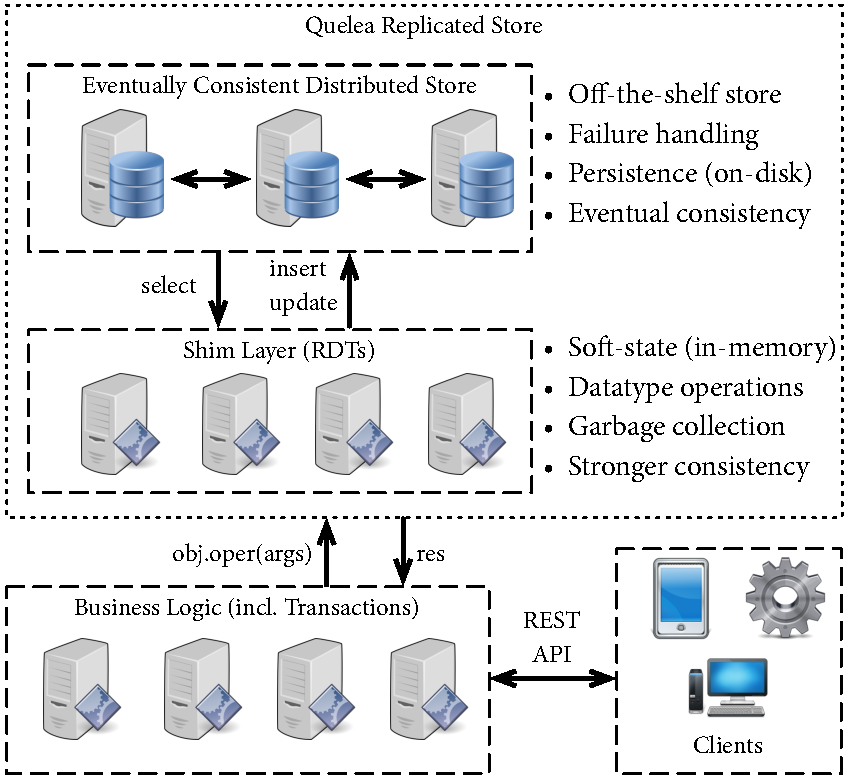
\includegraphics[width=0.7\columnwidth]{Figures/ImplModel}
\end{center}
\caption{Implementation Model.}
\label{fig:impl_mod}
\end{figure}

Replicated data types and the stronger consistency semantics are implemented
and enforced in the \emph{shim layer}. Our implementation supports eventual,
causal, and strong consistency for data type operations, and RC, MAV, and RR
semantics for transactions.  This functionality is implemented entirely on top
of the standard interface exposed by Cassandra. From an engineering
perspective, leveraging an off-the-shelf data store enables an implementation
comprising roughly only 2500 lines of Haskell code, packaged as a
library\footnote{url to the hackage}.

%% Complex business logic is implemented with the help of
%% transactions on the web-server side, with clients interacting with the
%% web-service over REST interface.

\subsection{Shim Layer}

The shim layer maintains a causally consistent in-memory snapshot of a subset
of objects in the backing store, by explicitly tracking dependencies introduced
between effects due to visibility, session and same transaction relations.
Dependence tracking is similar to the techniques presented in~\cite{BoltOn}
and~\cite{Eiger}. Because Cassandra provides durability, convergence and fault
tolerance, each shim layer node simply acts as a soft-state cache, do not
communicate directly with each other, and can safely be terminated at any point.
Similarly, new shim layer nodes can be spawned on demand.

The shim layer nodes periodically fetch updates from the store for eventually
consistent operations, and on-demand for causally consistent and strongly
consistent operations. Strongly consistent operations are performed after
obtaining exclusive leases on objects. The lease mechanism is implemented with
the help of Cassandra's support for conditional updates and expiring columns.

Cassandra does not provide general-purpose transactions. Since the transaction
guarantees provided by \name are coordination-free~\cite{BailisHAT}, we realize
efficient implementations by explicitly tracking the dependencies between
operations and transactions. Importantly, the weaker isolation semantics of
transactions in \name permit transactions to be discharged if at least one shim
layer node is reachable.

\subsection{Summarization}

The main challenge in realizing an efficient implementation of
operation-based replicated data types is that the state of the object
defined in terms of its set of effects, grows with every effectful
operation. If left unchecked, performance slow down over time, until the
shim layer memory or backing store disk runs out of memory. Luckily, the
state of the operation-based replicated data type can often be summarized to
an \emph{observably equivalent} smaller state. For example,

\begin{itemize}
\setlength{\itemsep}{2pt}
\item A last-writer-wins register with multiple updates where $v$ is the value
of the last write is observably equivalent to a register with a single write
$v$.

\item A bank account with a series of deposits and withdraws with current
balance $b$ is equivalent to a bank account with a single deposit of $b$.

\item A set with collection of add and remove operations is equivalent to a set
with a series of add operations of live elements from the original set.
\end{itemize}

\noindent Since the semantics of summarization depends on the semantics of the data
type, our programming model provides a summarization function for each RDT:
\begin{codehaskell}
summarize :: Effect e => [e] -> [e]
\end{codehaskell}
\noindent with the intention that the length of the result is smaller that the
length of the argument. We utilize the \cf{summarize} function to summarize the
object state both in the shim layer node and the backing store, typically when
the number of effects on an object crosses a tunable threshold. Shim layer
summarization is straight-forward; a summarization thread takes the local lock
on the object, and replaces its state with the summarized state. The shim layer
node remains unavailable for that particular object during summarization
(usually a few milliseconds).

Performing summarization in the backing store is more complicated since the whole
process needs to be atomic from a client's perspective, but Cassandra does not
provide multi-row transactions. We have implemented a highly available
implementation of summarization that permits concurrent client operations, but
nonetheless prohibits these operations from witnessing intermediate states of
the summarization process.
